\section{大型加速器実験}
加速器実験では、加速させた高エネルギーの粒子同士を衝突させることで、新たな粒子を作り出すことや、粒子同士の相互作用を観測することができる。

LHCは、図\ref{fg:LHC}にあるように1 周約27 kmの加速器である。

\begin{figure}[h]  %*** 図の挿入方法
    \centering
    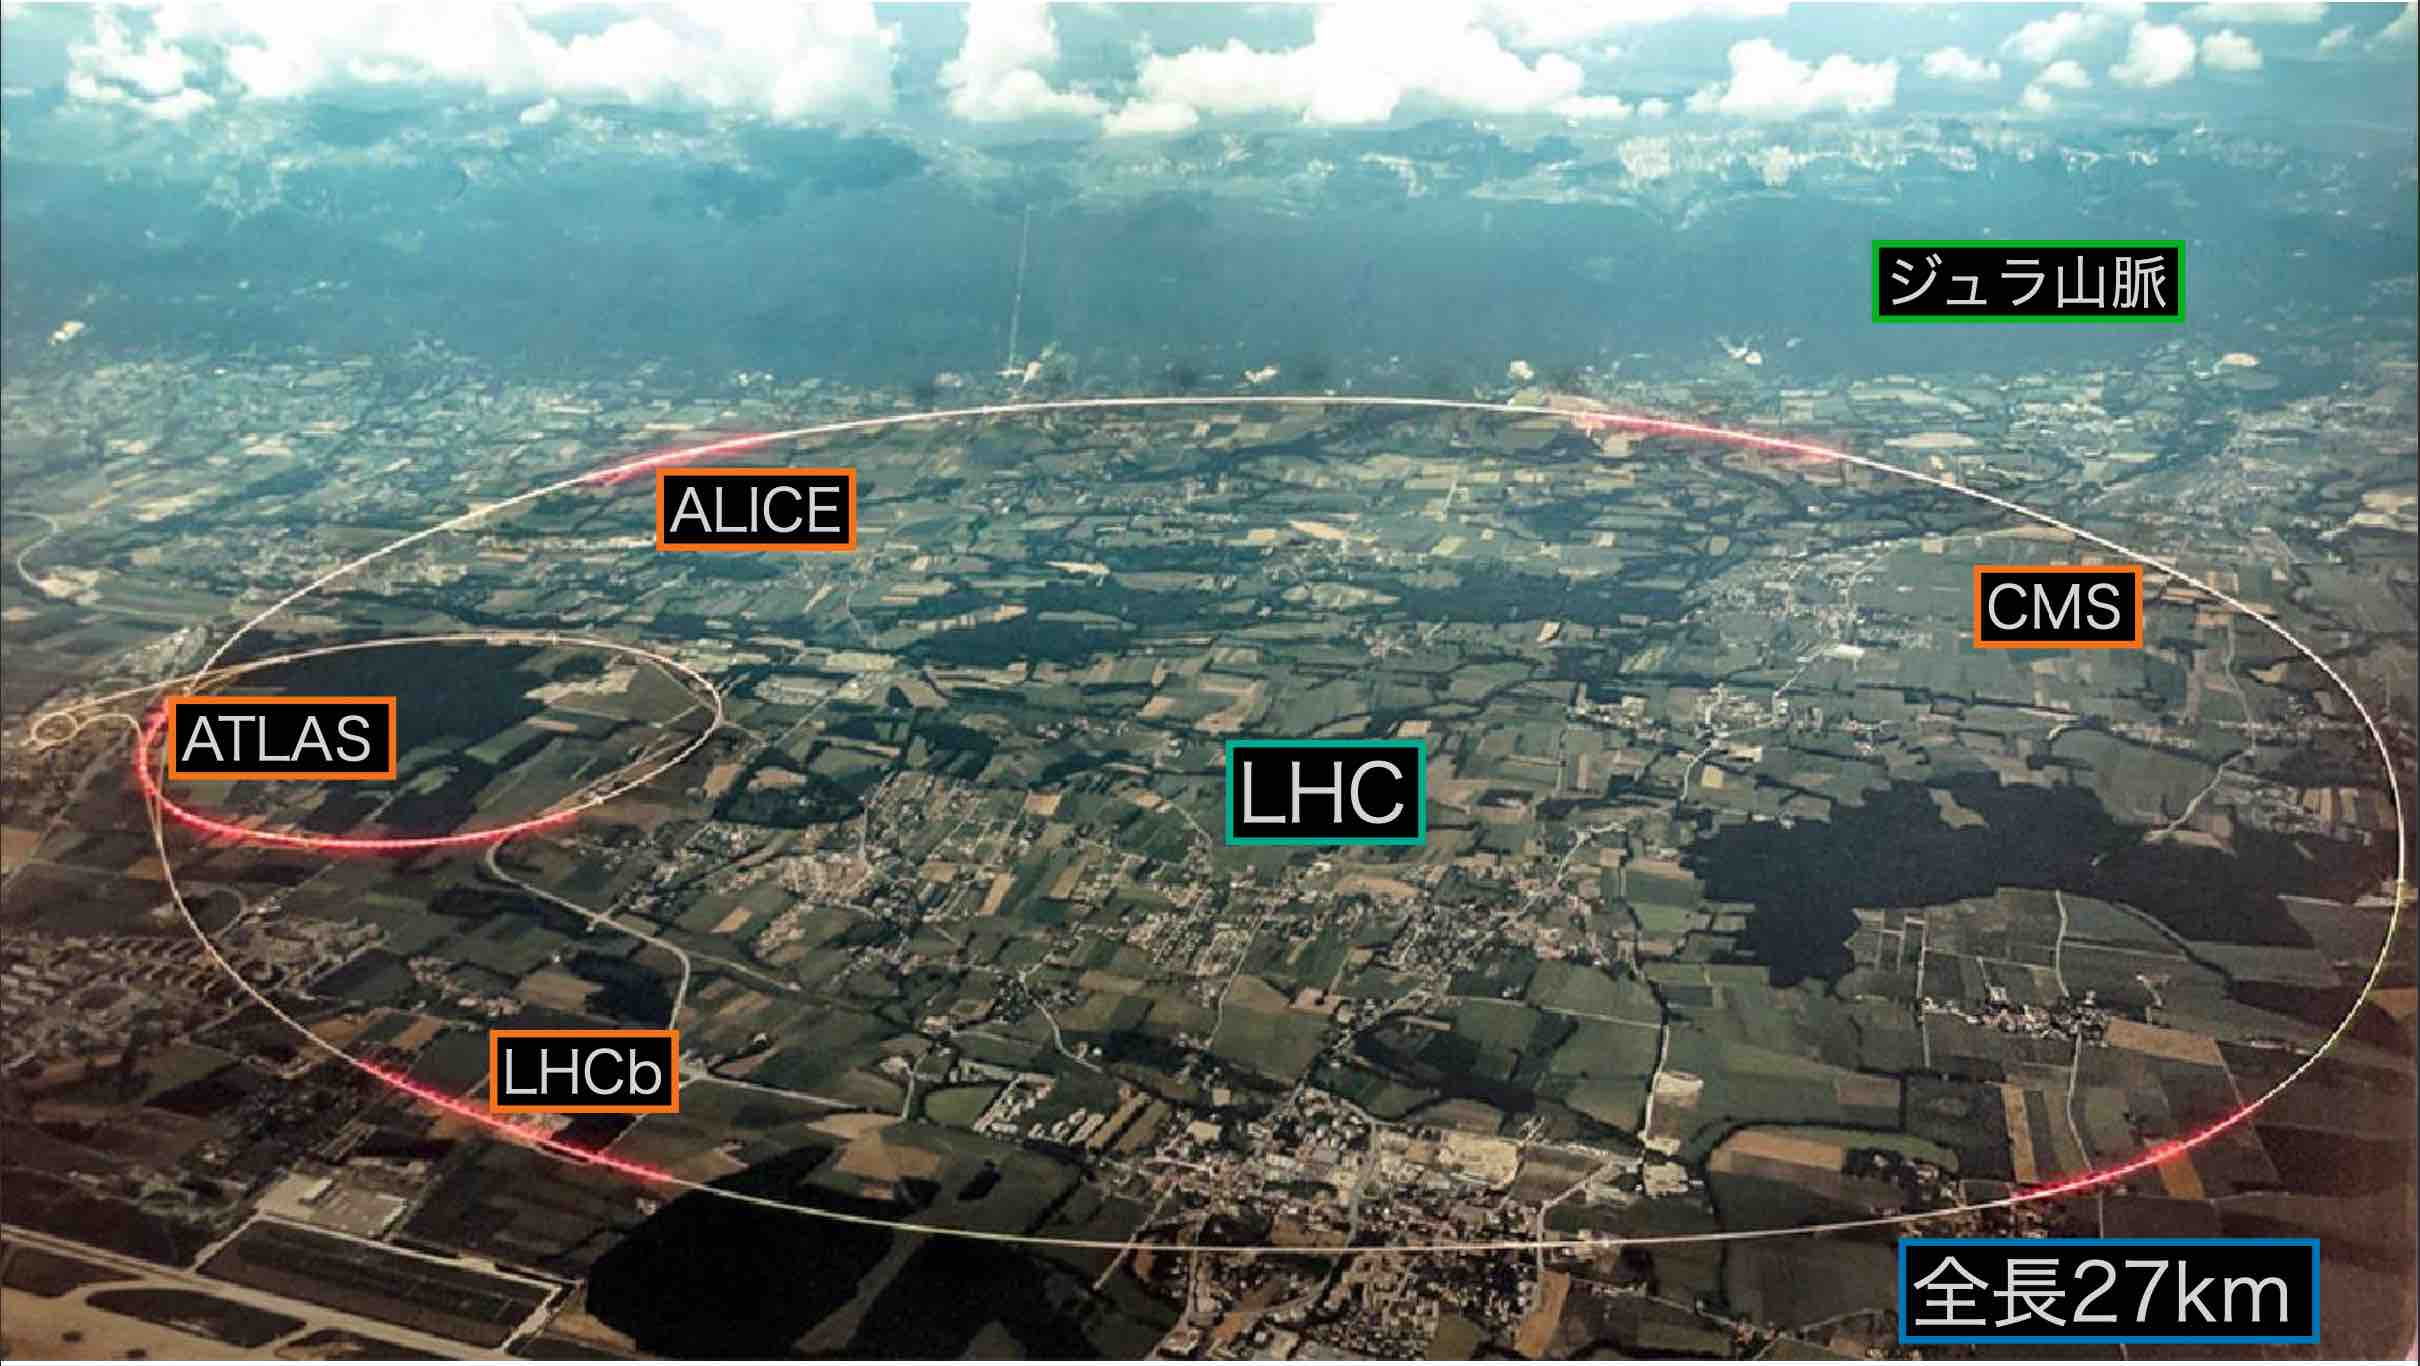
\includegraphics[width=12cm]{fig/ch1/LHC.jpg}
    \caption{Large Hadron Colider(LHC)の鳥瞰図\cite{LHCphoto}}
    \label{fg:LHC}
\end{figure}